\documentclass{article}
\usepackage[utf8]{inputenc}
\usepackage{amsmath}
\usepackage{amssymb}
\usepackage{mathtools}
\usepackage{halloweenmath}
\usepackage{graphicx}

\graphicspath{{Images/}}

\setlength{\oddsidemargin}{0in}
\setlength{\textwidth}{6.5in}
\setlength{\topmargin}{-.55in}
\setlength{\textheight}{9in}
\pagestyle{empty}



\title{Solid State Physics HW 6}
\author{Michael Nameika}
\date{October 2022}

\begin{document}

\maketitle

\section*{Problem 1}
Consider a chain of identical atoms of mass $M$ with nearest neighbor coupling separated by the distance "$a$". The force constants have values $C_1$ and $C_2$ ($C_1 > C_2$), such that each atom is coupled to one neighbor with $C_1$ and to the other with $C_2$. Find the equation of motion and dispersion relations (plot them). What is the difference with a diatomic chain with alternating masses $M_1$ and $M_2$ but equal force constants?
\newline\newline
We find the following coupled set of differential equations that related the equation of motion to the nearest neighbors:
\begin{align*}
    M\frac{d^2u_s}{dt^2} &= C_1(v_s - u_s) + C_2(v_{s-1} - u_s) \\
    M\frac{d^2v_s}{dt^2} &= C_1(u_s - v_s) + C_2(u_{s+1} - v_s) \\
\end{align*}
We seek solutions of the form 
\begin{align*}
    u_s &= ue^{i(2kas - \omega t)} \\
    v_s &= ve^{i(2kas - \omega t)} \\
\end{align*}
Using these in our coupled differential equations, we find
\begin{align*}
    -M\omega^2u &= C_1(v - u) + C_2(ve^{-i2Ka} - u) \\
    -M\omega^2v &= C_1(u - v) + C_2(ue^{i2Ka} - v) \\
\end{align*}
Writing as a linear system, we have
\[\begin{bmatrix}
    -M\omega^2 + C_1 + C_2 & -(C_1 + C_2)e^{-i2Ka} \\
    -(C_1 + C_2)e^{i2Ka} & -M\omega^2 + C_1 + C_2 \\
\end{bmatrix}
\begin{bmatrix}
    u\\
    v\\
\end{bmatrix}
=
\begin{bmatrix}
    0\\
    0\\
\end{bmatrix}\]
Then we require the determinant of the above matrix to be zero to find nontrivial solutions, which leads us to
\[(C_1 + C_2 - M\omega^2)^2 - (C_1 + C_2e^{-i2Ka})(C_1 + C_2e^{i2Ka}) = 0\]
Which leads us to the following solutions:
\[M\omega^2 = (C_1 + C_2) \pm \left(C_1^2 + C_2^2 + 2C_1C_2\cos{(2Ka)}\right)^{1/2}\]
I was unable to figure out how to remove the dependence of $C_1$ and $C_2$ on the right hand side of the above equation, so I used specific values of $C_1$ and $C_2$ to plot the dispersion relation to get a general sense of the shape.
\begin{center}
    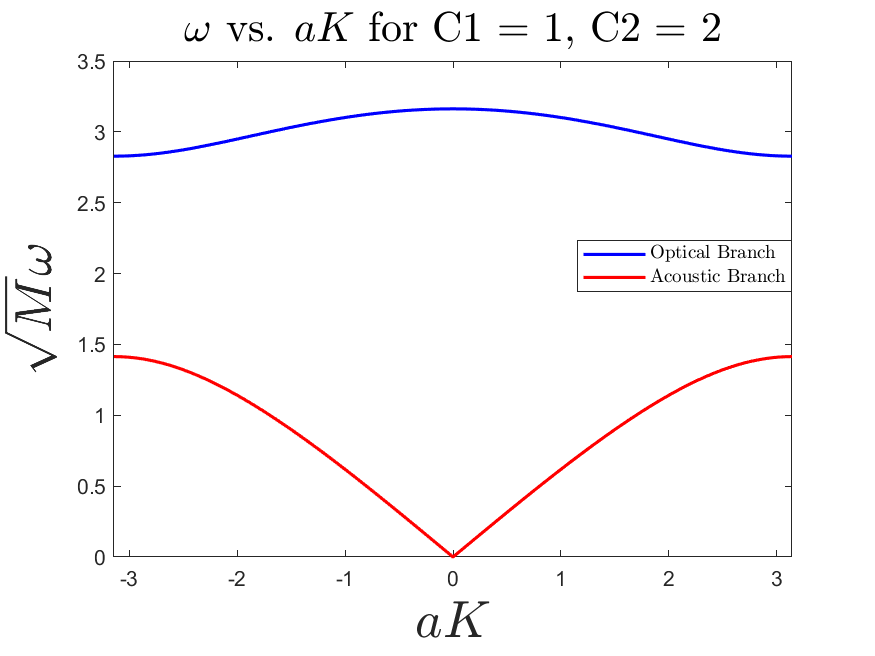
\includegraphics[scale = 0.6]{optical vs acoustic.png}
\end{center}
The difference with a diatomic chain with the same force constants and different masses is that the optical branch for a diatomic chain with identical force constants and different masses is constant and the acoustic branch takes the form of a quadratic function. For our atomic chain, this relationship is similar, but we can see some variability in the optical branch.

See attached sketches and work for additional details.

\section*{Problem 4.1}
\textit{\textbf{Monatomic linear lattice.}} Consider a longitudinal wave
\[u_s = u\cos{(\omega t - sKa)}\]
which propagates in a monatomic linear lattice of atoms of mass $M$, spacing $a$, and nearest-neighbor interaction $C$.
(a) Show that the total energy of the wave is
\[E = \frac{1}{2}M\sum_s(du_s/dt)^2 + \frac{1}{2}C\sum_s(u_s - u_{s+1})^2.\]
where $s$ runs over all atoms. 
\newline
(b) By substitution of $u_s$ in this expression, show that the time-average total energy per atom is 
\[\frac{1}{4}M\omega^2u^2 + \frac{1}{2}C(1-cos(Ka)u^2 = \frac{1}{2}M\omega^2u^2\]
where in the last step we have used the dispersion relation (9) for this problem.
\newline\newline
(a) Recall that the total energy of a system is the sum of the kinetic and potential energy. In our case, the kinetic energy is the 'usual' $1/2mv^2$ and our potential energy is the spring potential since our system takes the form of Hooke's law. Our velocity is
\[v_s = \frac{du_s}{dt}\]
and our potential energy takes the form of
\[PE_s = \frac{1}{2}C(u_s - u_{s+1})^2\]
Then summing over every atom in the crystal, we have
\[E = \frac{1}{2}M\sum_{s}\left(\frac{du_s}{dt}\right)^2 + \frac{1}{2}C\sum_{s}(u_s - u_{s+1})^2\]
Which is what we wanted to show.
\newline\newline
(b) Since we are only looking at the time average of of the energy per atom, we need not look at the entire summation we found in part (a). Since our displacement is given by $u_s = u\cos{(\omega t - sKa)}$, 
\begin{align*}
    &v_s = \frac{du_s}{dt} = -\omega u \sin{(\omega t - sKa)}\\
    &\left(\frac{du_s}{dt}\right)^2 = \omega^2u^2\sin^2{(\omega t - sKa)} \\
\end{align*}
and so the time average of the velocity squared is
\[\langle v^2 \rangle = \frac{1}{2}\omega^2u^2\]
And so our average kinetic energy is
\[\langle KE_s \rangle  = \frac{1}{4}M\omega^2u^2\]
Now, we have for our potential energy,
\begin{align*}
    \frac{1}{2}C(u_s - u_{s+1})^2 &= \frac{1}{2}C(u\cos{(\omega t - sKa) - u\cos{(\omega t - (s+1)Ka)}})\\
    &= \frac{1}{2}C(u^2\cos^2{(\omega t - sKa)} + u^2\cos^2{(\omega t - (s+1)Ka)} - 2u^2\cos{(\omega t - sKa)}\cos{(\omega t - (s+1)Ka)}) \\
    &=\frac{1}{2}C(u^2cos^2{(\omega t - sKa)} + u^2\cos^2{(\omega t - (s+1)Ka)} - (u^2(\cos{(2\omega t -2sKa - Ka)} + \cos{(Ka)})) \\
\end{align*}
And taking the time average, we see
\begin{align*}
    \langle 1/2C(u_s - u_{s+1})^2 \rangle &= \frac{1}{2}C\left(\frac{1}{2}u^2 + \frac{1}{2}u^2 + u^2\cos{(Ka)}\right) \\
    &= \frac{1}{2}Cu^2(1 - \cos{(Ka)}) \\
    &= \frac{1}{4}Cu^2\sin^2{(Ka/2)} \\
\end{align*}
and from the dispersion relation (9), we have
\begin{align*}
    \langle 1/2C(u_s - u_{s+1})^2 \rangle = \frac{1}{4}M\omega^2 \\
\end{align*}
Putting it together, we have for the time average of the total energy,
\begin{align*}
    \langle E \rangle = \frac{1}{2}M\omega^2u^2 \\
\end{align*}

\section*{Problem 4.2}
\textit{\textbf{Continuum wave equation.}} Show that for long wavelengths the equation of motion (2) reduces to the continuum elastic wave equation
\[\frac{\partial^2 u}{\partial t^2} = v^2\frac{\partial^2u}{\partial x^2}\]
where $v$ is the velocity of sound.
\newline\newline
From equation (2), we have
\[M\frac{d^2u_s}{dt^2} = C(u_{s+1} + u_{s-1} - 2u_s)\]
Notice that the right hand side is the form of a second order difference equation of the second derivative of $u$ with respect to displacement. Then we can rewrite the above equation as
\begin{align*}
    \frac{\partial^2u_s}{\partial t^2} = \frac{C}{M}a^2\frac{\partial^2u_s}{\partial x^2} \\
\end{align*}
where $a$ is the distance between displaced planes. This is the 1-D wave equation with $v^2 = C/Ma^2$.


\section*{Problem 4.3}
\textit{\textbf{Basis of two unlike atoms.}} For the problem treated by (18) to (26), find the amplitude ratios $u/v$ for the two branches at $K_{\text{max}} = \pi/a$. Show that at this value of $K$ the two lattices act as if decoupled: one lattice remains at rest while the other lattice moves.
\newline\newline
To begin, recall that we require the following equation to hold for $\omega$:
\[M_1M_2\omega^4 - 2c(M_1 + M_2)\omega^2 + 2C^2(1 - \cos{(Ka)}) = 0\]
Then using the quadratic formula to solve for $\omega^2$, we have (when $K = \pi/a$):
\begin{align*}
    \omega^2 &= \frac{2C(M_1 + M_2) \pm \sqrt{4C^2(M_1 + M_2)^2 - 16C^2M_1M_2}}{2M_1M_2} \\
    &= \frac{2C(M_1 + M_2) \pm 2C\sqrt{M_1^2 + 2M_1M_2 + M_2^2 - 4M_1M_2}}{2M_1M_2} \\
    &= \frac{2C(M_1 + M_2) \pm 2C\sqrt{M_1^2 - 2M_1M_2 + M_2^2}}{2M_1M_2} \\
    &= \frac{2C(M_1 + M_2) \pm 2C(M_1 - M_2)}{2M_1M_2} \\
\end{align*}
So our values for $\omega^2$ are 
\begin{align*}
    \omega^2 &= \frac{2C}{M_1} \\
    \text{or} \\
    \omega^2 &= \frac{2C}{M_2} \\
\end{align*}
Now, from equation (20), we have have the following relationship between $u$ and $v$:
\[u = \frac{Cv(1 + \exp{(-iKa)})}{2C - \omega^2M_1}\]
Then for $K = \pi/a$:
\begin{align*}
    \frac{u}{v} &= \frac{C(1 + \exp{(-i\pi)})}{2C - \omega^2M_1} \\
    &= 0 \\
\end{align*}
Then we have $u = 0$ and $v \neq 0$. So from equation (19), we have
\begin{align*}
    u_s &= 0\\
    v_s &= \pm v\exp{(-i\omega t)} \\
\end{align*}
That is, one lattice remains at rest while the other lattice moves. Finally, to show the two are decoupled, notice that equation (20) becomes, when $K = \pi/a$,
\begin{align*}
    -\omega^2M_1u &= -2Cu\\
    -\omega^2M_2v &= -2Cv\\
\end{align*}
which shows us that the $u$ and $v$ are decoupled and depend only on themselves.


\section*{Problem 4.4}
\textit{\textbf{Kohn anomaly}}. We suppose that the interplanar force constant $C_p$ between planes $s$ and $s + p$ is of the form
\[C_p = A\frac{\sin{(pk_0a)}}{pa}\]
where $A$ and $k_0$ are constants and $p$ runs over all integers. Such a form is expected in metals. Use this and Eq. (16a) to find an expression for $\omega^2$ and also for $\partial \omega^2/\partial K$. Prove that $\partial \omega^2/\partial K$ is infinite when $K = k_0$. Thus a plot of $\omega^2$ versus $K$ or of $\omega$ versus $K$ has a vertical tangent at $k_0$: there is a kink at $k_0$ in the phonon dispersion relation $\omega(K)$.
\newline\newline
Plugging this constant into equation (16a), we find the following:
\begin{align*}
    \omega^2 &= (2/M)\sum_{p > 0}\frac{A\sin{(pk_0a)}}{pa}(1 - \cos{(pKa)}) \\
    &= \frac{2A}{Ma}\sum_{p > 0}\frac{\sin{(pk_0a)}}{p}(1 - \cos{(pKa)}) \\
\end{align*}
Taking the first partial with respect to K, we find
\begin{align*}
    \frac{\partial\omega^2}{\partial K} &= \frac{2A}{Ma}\sum_{p > 0}\sin{(pk_0a)}\sin{(pKa)}\\
    &= \frac{2A}{Ma}\sum_{p > 0}\sin{(pKa)}\sin{(pk_0a)} \\
\end{align*}
Then when $K = k_0$, we have
\begin{align*}
    \frac{\partial\omega^2}{\partial K} &= \frac{2A}{Ma}\sum_{p > 0}\sin^2{(pk_0a)} \\
    &= \frac{2A}{M}\sum_{p > 0} \sin^2{(pk_0a)} \\
\end{align*}
We must show that $\sum_{p > 0}\sin^2{(pk_0a)}$ diverges. Well, so long as $k_0a \neq n\pi, n \in \mathbb{Z}$, we have 
\[\lim_{p \to \infty} \sin^2{(pk_0a)} \:\: \text{DNE}\]
and so by the test for divergence, $\sum_{p > 0} \sin^2{(pk_0a)}$ diverges. That is, when we are within the boundaries of the first Brillouin zone (and not at $k_0 = 0$), we have $\omega^2$ has a vertical tangent at $k_0$.
\newline\newline\newline
Carrying out the summation for one thousand terms for 50 points between $0$ and $\pi$ for $A = 1/2$, $a = 1$, $M = 1$, and $k_0 = \pi/(3a)$, we find the following plot of $\omega^2$ vs $K$:
\begin{center}
    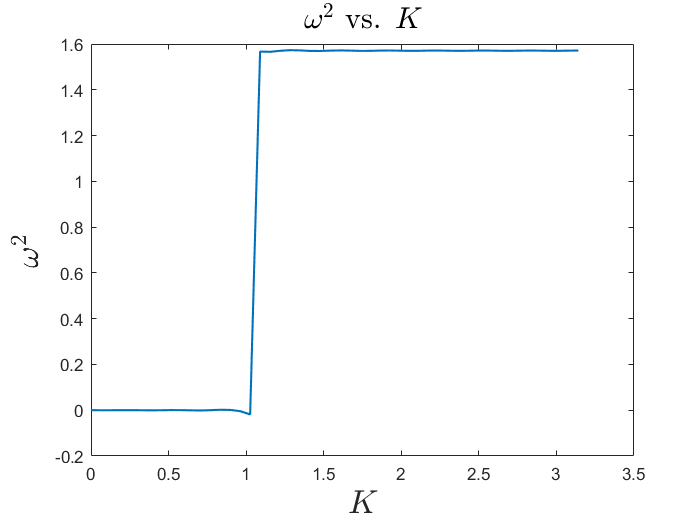
\includegraphics[scale = 0.6]{omegasqrvsk.png}
\end{center}

\end{document}
